% The Mid-Context Dead Zone in KV Cache Compression
% Measurement-first framing. The specification-first framing of the same
% evidence is paper.tex; both share figure.tex and refs.bib.
%
% Build:  pdflatex paper-measurement && bibtex paper-measurement && \
%         pdflatex paper-measurement && pdflatex paper-measurement
\documentclass[10pt]{article}
\usepackage[margin=1in]{geometry}
\usepackage[T1]{fontenc}
\usepackage[utf8]{inputenc}
\usepackage{booktabs}
\usepackage{amsmath}
\usepackage{tikz}
\usepackage{xcolor}
\usepackage{natbib}
\usepackage[hidelinks]{hyperref}
\usepackage{microtype}

\definecolor{tealaccent}{HTML}{0E7C86}
\definecolor{rustaccent}{HTML}{B0541F}

\title{The Mid-Context Dead Zone in KV Cache Compression}
\author{Srujan Pendurthi\\\texttt{srujan.pendurthi@gmail.com}}
\date{}

\begin{document}
\maketitle

\begin{abstract}
KV cache compression is evaluated on aggregate accuracy at a given budget,
which hides \emph{where} in the context a method succeeds. Measuring recall
against distance from the query, we find the token-scoring rules published
methods are built on partition the context by position rather than utility:
recency scoring recovers only the near field, accumulated-attention scoring
only the far field, and \textbf{no rule we tested recovers the middle at any
budget}---0 successes in 340 middle-band trials across three models spanning a
$4.7\times$ size range (95\% upper bound 0.9\%), against an uncompressed cache
that answers all of them.

We give the mechanism. Admission at rate $p$ followed by FIFO eviction to
budget $B$ leaves a contiguous window over the most recent $B/p$ positions, so
retention is a \textbf{step function with a hard horizon}: beyond it, survival
is exactly zero rather than merely unlikely. Recency is emergent rather than
chosen---any rule that does not actively protect distant tokens decays onto it.

An \textbf{oracle retention} control---identical budget, chunking and eviction,
but told which tokens carry the answers---scores $40/40$ at 1.7B and $24/24$ at
8B, matching the uncompressed cache on a quarter of the context. \textbf{The
dead zone is not a capacity limit but an observability one}, and we give the
specification a realisable signal must meet, then use it as a screening test
that rejects ten candidates across eight framings---one for \$0,
with its end-to-end failure predicted in advance.

Finally we isolate a second constraint: at fixed evidence, distance, budget and
recency fill, \textbf{splitting the retained set into more pieces destroys
recall} ($0.54$ at eight fragments against $0.92$ at four, $p{=}0.008$).
\end{abstract}

\section{Introduction}

A long-context model writes every token into its KV cache; under a budget most
must go. The literature decides what to discard by ranking tokens with
attention-derived rules---accumulated attention \citep{zhang2023h2o},
observation-window voting \citep{li2024snapkv}, recency plus attention sinks
\citep{xiao2024streamingllm}, layer-wise budget allocation
\citep{cai2024pyramidkv,feng2024adakv}---and reports aggregate accuracy at a
compression ratio.

Those methods differ in engineering, but the component deciding \emph{what to
keep} is in each case a token-scoring rule, and that is what we isolate. The
aggregate metric cannot distinguish a rule that retains information uniformly
from one that retains a biased subset well. We ask a narrower question:
\textbf{given a fact planted at distance $d$ before the query, does the
compressed cache still support answering it?}

\paragraph{Contributions.}
\begin{enumerate}\itemsep2pt
\item A \textbf{distance-resolved measurement} showing published scoring rules
      partition context by position---recency and attention-accumulation
      recovering \emph{complementary} halves---and that a mid-context dead zone
      survives every rule, budget, model and task tried
      (\S\ref{sec:deadzone}). Position-resolved evaluation of compression
      exists (\S\ref{sec:related}); the complementarity and the systematic zero
      do not.
\item A \textbf{mechanism}---a hard retention horizon at $d = B/p$---predicting
      \texttt{recent} exactly and explaining why recency is emergent
      (\S\ref{sec:mech}).
\item An \textbf{oracle control} establishing the dead zone is observability,
      not capacity, at two model scales (\S\ref{sec:oracle}).
\item A \textbf{specification} for what a realisable signal must achieve and
      its use as a cheap \textbf{screening test}; ten candidates rejected, one
      with its end-to-end failure predicted from a \$0 measurement
      (\S\ref{sec:spec}, \S\ref{sec:screen}).
\item A \textbf{controlled isolation of fragmentation}---at matched evidence,
      distance and budget---attributing the effect to the \emph{number} of
      contiguous runs rather than their length (\S\ref{sec:frag}). The
      phenomenon itself is known (\S\ref{sec:related}).
\end{enumerate}

\section{Setup and scope}\label{sec:setup}

\textbf{Models.} Qwen3-1.7B (primary), SmolLM2-1.7B-Instruct and Qwen3-8B;
bf16, frozen. No model weights are trained anywhere in this work.
\textbf{Streams.} \emph{Synthetic:} 8192 tokens of prose with eight facts
\texttt{The secret code for <topic> is <6 digits>} at evenly spaced, per-seed
jittered anchors, each queried from the end. \emph{Real:} 8192 tokens of
distractor SQuAD paragraphs with eight gold paragraphs planted at the same
anchors, queried by their human-written questions; distractors are drawn only
from articles no gold paragraph belongs to.
\textbf{Compression.} Chunked prefill at 128 tokens, compressed to budget $B$
per layer after each chunk, first four tokens pinned as sinks. Budgets
256/512/1024/2048.
\textbf{Metrics.} Exact substring match on the synthetic task; containment plus
token F1 on real QA against a measured closed-book floor. Zero-hit cells report
a rule-of-three upper bound rather than a standard error.
\textbf{Banding.} Near/middle/far terciles of distance-back from the query.

\paragraph{What the baselines are, precisely.}
\texttt{recent}, \texttt{h2o} and \texttt{snapkv} implement the
\emph{token-scoring rule} of StreamingLLM, H2O and SnapKV---recency plus sinks,
accumulated attention mass, observation-window voting---at token granularity
under a uniform per-layer budget. They are \textbf{not} reproductions of those
systems: no per-head budgets, no layer-wise allocation, none of the kernel and
memory engineering those papers contribute. Absolute numbers are not comparable
to published ones and nothing here benchmarks a published system. What is under
test is the scoring rule, because that is the component the dead zone is a
property of.

\paragraph{Harness correctness.} At unbounded budget, logits are bit-identical
to a stock \texttt{DynamicCache} under the same chunking, verified on two
backends. Positions are passed explicitly, since compression makes cache length
diverge from stream position---a silent corruption otherwise. 135 tests.

\section{The dead zone}\label{sec:deadzone}

Per-rule recall at $B{=}2048$, a quarter of the stream, on Qwen3-1.7B:

\begin{table}[h]\centering\small
\begin{tabular}{lccc}
\toprule
rule & near & middle & far \\
\midrule
\texttt{recent} & $\mathbf{10/14}$ & $0/12$ & $\mathbf{0/14}$ \\
\texttt{random} & $7/14$ & $0/12$ & $0/14$ \\
\texttt{snapkv} & $4/14$ & $0/12$ & $0/14$ \\
\texttt{h2o}    & $\mathbf{0/14}$ & $0/12$ & $\mathbf{8/14}$ \\
\texttt{full}   & 1.00 & 1.00 & 1.00 \\
\bottomrule
\end{tabular}
\end{table}

\texttt{recent} and \texttt{h2o} are exact complements: each scores strongly in
one band and \emph{exactly} zero in the other, and neither reaches the middle.
This follows from the rules themselves. Accumulated attention sums over query
rows, and the earliest tokens are visible to the most of them, so it leans
toward the start by construction, as recency leans toward the end.
\textbf{Both are functions of position; neither is a function of utility.}

\paragraph{Across models.} The same sweep on SmolLM2-1.7B gives $0/56$ in the
middle band against an uncompressed $7/7$. On Qwen3-8B---same family as the
primary model, so scale is the only variable---$0/56$ against a ceiling perfect
in all three bands, with the complementarity intact (\texttt{recent} $6/9$ near
and $0/8$ far; \texttt{h2o} $0/9$ near and $4/8$ far). Pooled: \textbf{0 of 340
middle-band trials}, 95\% upper bound 0.9\%.

\paragraph{On real QA.} Replacing the synthetic task with planted-evidence
SQuAD---human-written questions, natural-language answers, containment plus F1
against a measured \textbf{closed-book floor of $0/24$}---gives $1/64$ in the
middle band (95\% upper 7.2\%) against an uncompressed $6/8$. The single hit is
\texttt{h2o} at $d{=}4729$, gold \emph{rivers}, generated \emph{certain
rivers}; the closed-book control confirms retrieval rather than a guess. Two
caveats are specific to that task: its far band has a difficulty ceiling
(\texttt{full} scores $4/7$), so far-band zeros there are weak evidence; and it
discriminates only on Qwen3-1.7B---on SmolLM2 the uncompressed ceiling is
$11/24$ against a $3/24$ floor, an eight-trial window in which nothing
separates.

\paragraph{Why this does not rest on baseline fidelity.} Three parts of the
argument are independent of whether our rules match the published systems. The
ceiling is \emph{measured}, not assumed: \texttt{full} uses the same harness and
answers everything. The oracle (\S\ref{sec:oracle}) is measured at the
\emph{same budget} through the \emph{same} eviction path and answers
everything, so a 2048-token cache built by this harness can reach the middle.
And the mechanism (\S\ref{sec:mech}) is geometric, holding exactly for
\texttt{recent}, whose rule has no implementation freedom worth disputing. A
faithful reimplementation could move the near- and far-band numbers; it could
not move the middle without replacing the scoring rule.

\section{Mechanism: a hard horizon}\label{sec:mech}

\begin{figure}[t]
\centering
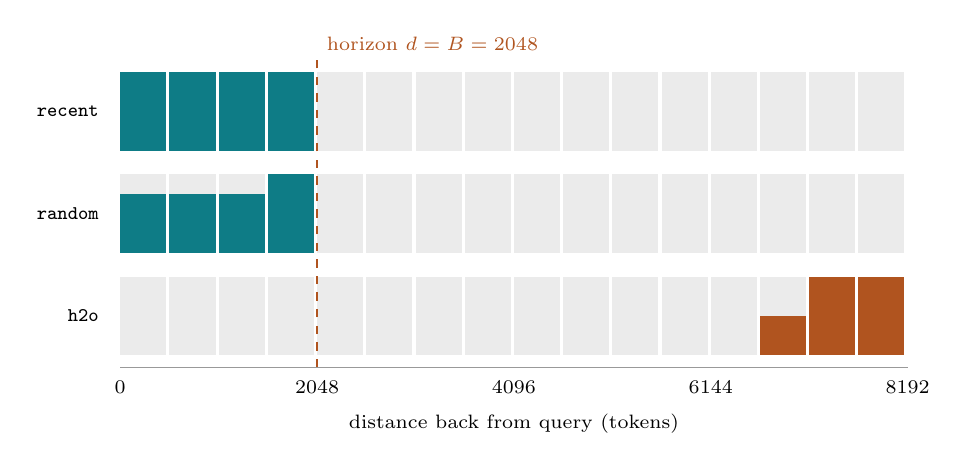
\begin{tikzpicture}[x=1cm,y=1cm]
% recent
    \fill[black!8] (0.000,2.60) rectangle ++(0.585,1.0);
    \fill[tealaccent] (0.000,2.60) rectangle ++(0.585,1.000);
    \fill[black!8] (0.625,2.60) rectangle ++(0.585,1.0);
    \fill[tealaccent] (0.625,2.60) rectangle ++(0.585,1.000);
    \fill[black!8] (1.250,2.60) rectangle ++(0.585,1.0);
    \fill[tealaccent] (1.250,2.60) rectangle ++(0.585,1.000);
    \fill[black!8] (1.875,2.60) rectangle ++(0.585,1.0);
    \fill[tealaccent] (1.875,2.60) rectangle ++(0.585,1.000);
    \fill[black!8] (2.500,2.60) rectangle ++(0.585,1.0);
    \fill[black!8] (3.125,2.60) rectangle ++(0.585,1.0);
    \fill[black!8] (3.750,2.60) rectangle ++(0.585,1.0);
    \fill[black!8] (4.375,2.60) rectangle ++(0.585,1.0);
    \fill[black!8] (5.000,2.60) rectangle ++(0.585,1.0);
    \fill[black!8] (5.625,2.60) rectangle ++(0.585,1.0);
    \fill[black!8] (6.250,2.60) rectangle ++(0.585,1.0);
    \fill[black!8] (6.875,2.60) rectangle ++(0.585,1.0);
    \fill[black!8] (7.500,2.60) rectangle ++(0.585,1.0);
    \fill[black!8] (8.125,2.60) rectangle ++(0.585,1.0);
    \fill[black!8] (8.750,2.60) rectangle ++(0.585,1.0);
    \fill[black!8] (9.375,2.60) rectangle ++(0.585,1.0);
  \node[anchor=east,font=\scriptsize\ttfamily] at (-0.15,3.1) {recent};
% random
    \fill[black!8] (0.000,1.30) rectangle ++(0.585,1.0);
    \fill[tealaccent] (0.000,1.30) rectangle ++(0.585,0.750);
    \fill[black!8] (0.625,1.30) rectangle ++(0.585,1.0);
    \fill[tealaccent] (0.625,1.30) rectangle ++(0.585,0.750);
    \fill[black!8] (1.250,1.30) rectangle ++(0.585,1.0);
    \fill[tealaccent] (1.250,1.30) rectangle ++(0.585,0.750);
    \fill[black!8] (1.875,1.30) rectangle ++(0.585,1.0);
    \fill[tealaccent] (1.875,1.30) rectangle ++(0.585,1.000);
    \fill[black!8] (2.500,1.30) rectangle ++(0.585,1.0);
    \fill[black!8] (3.125,1.30) rectangle ++(0.585,1.0);
    \fill[black!8] (3.750,1.30) rectangle ++(0.585,1.0);
    \fill[black!8] (4.375,1.30) rectangle ++(0.585,1.0);
    \fill[black!8] (5.000,1.30) rectangle ++(0.585,1.0);
    \fill[black!8] (5.625,1.30) rectangle ++(0.585,1.0);
    \fill[black!8] (6.250,1.30) rectangle ++(0.585,1.0);
    \fill[black!8] (6.875,1.30) rectangle ++(0.585,1.0);
    \fill[black!8] (7.500,1.30) rectangle ++(0.585,1.0);
    \fill[black!8] (8.125,1.30) rectangle ++(0.585,1.0);
    \fill[black!8] (8.750,1.30) rectangle ++(0.585,1.0);
    \fill[black!8] (9.375,1.30) rectangle ++(0.585,1.0);
  \node[anchor=east,font=\scriptsize\ttfamily] at (-0.15,1.8) {random};
% h2o
    \fill[black!8] (0.000,0.00) rectangle ++(0.585,1.0);
    \fill[black!8] (0.625,0.00) rectangle ++(0.585,1.0);
    \fill[black!8] (1.250,0.00) rectangle ++(0.585,1.0);
    \fill[black!8] (1.875,0.00) rectangle ++(0.585,1.0);
    \fill[black!8] (2.500,0.00) rectangle ++(0.585,1.0);
    \fill[black!8] (3.125,0.00) rectangle ++(0.585,1.0);
    \fill[black!8] (3.750,0.00) rectangle ++(0.585,1.0);
    \fill[black!8] (4.375,0.00) rectangle ++(0.585,1.0);
    \fill[black!8] (5.000,0.00) rectangle ++(0.585,1.0);
    \fill[black!8] (5.625,0.00) rectangle ++(0.585,1.0);
    \fill[black!8] (6.250,0.00) rectangle ++(0.585,1.0);
    \fill[black!8] (6.875,0.00) rectangle ++(0.585,1.0);
    \fill[black!8] (7.500,0.00) rectangle ++(0.585,1.0);
    \fill[black!8] (8.125,0.00) rectangle ++(0.585,1.0);
    \fill[rustaccent] (8.125,0.00) rectangle ++(0.585,0.500);
    \fill[black!8] (8.750,0.00) rectangle ++(0.585,1.0);
    \fill[rustaccent] (8.750,0.00) rectangle ++(0.585,1.000);
    \fill[black!8] (9.375,0.00) rectangle ++(0.585,1.0);
    \fill[rustaccent] (9.375,0.00) rectangle ++(0.585,1.000);
  \node[anchor=east,font=\scriptsize\ttfamily] at (-0.15,0.5) {h2o};
% horizon
  \draw[rustaccent,dashed,thick] (2.500,-0.15) -- (2.500,3.75);
  \node[anchor=south west,font=\scriptsize,rustaccent] at (2.500,3.75)
    {horizon $d=B=2048$};
% axis
  \draw[black!40] (0,-0.15) -- (10,-0.15);
  \foreach \f/\l in {0/0, 0.25/2048, 0.5/4096, 0.75/6144, 1.0/8192}
    \node[anchor=north,font=\scriptsize] at ({\f*10},-0.2) {\l};
  \node[anchor=north,font=\scriptsize] at (5,-0.62)
    {distance back from query (tokens)};
\end{tikzpicture}
\caption{\textbf{The retention horizon.} Recall in 512-token distance bins at
$B{=}2048$ (Qwen3-1.7B, 4 seeds $\times$ 16 needles); bar height is recall,
grey is the empty cell. \texttt{recent} holds $1.00$ out to $d{=}B$ and
scores nothing beyond it; \texttt{h2o} is the mirror image anchored to
the start of the stream. Neither reaches the ${\approx}4000$ tokens between
them.}
\label{fig:horizon}
\end{figure}

Sixteen needles per stream, four seeds, $B{=}2048$, chunk 128, binned at
256-token resolution: \texttt{recent} scores $16/16$ below 2048 and $0/48$
above; \texttt{random} $13/16$ and $0/48$; \texttt{h2o} $0/16$ and $10/48$, all
at $d > 6600$. Under admission at rate $p$ followed by FIFO eviction to budget
$B$, occupancy saturates and the cache becomes a contiguous window over the
most recent $B/p$ raw positions:
\begin{equation}
  P(\text{token resident at distance } d) =
  \begin{cases} p & d < B/p \\ 0 & \text{otherwise.}\end{cases}
  \label{eq:horizon}
\end{equation}
\texttt{recent} ($p{=}1$) is predicted exactly. Tested at $p{=}0.5$, where the
horizon should move to 4096: $2/32$ inside, $0/32$ beyond---the horizon holds; the plateau is
$p^L$ rather than $p$, since recall needs every token of an $L$-token answer
(\S\ref{sec:limits}).

The claim this sharpens is not that distant tokens are unlikely to survive but
that \textbf{beyond the horizon they survive with probability exactly zero}, so
any rule that does not explicitly protect a token past $B/p$ loses it with
certainty. The middle band lies entirely beyond the horizon at every budget
tested. Compression is not a ranking problem but a rescue problem.
\texttt{h2o} has the mirror-image horizon (Fig.~\ref{fig:horizon}).

\section{Capacity exists: the oracle}\label{sec:oracle}

\textbf{Oracle retention} uses the identical budget, chunking, sink prefix,
FIFO eviction and evaluation, through the same eviction path as every baseline.
One thing changes: it is told which token spans carry the answers.

\begin{table}[h]\centering\small
\begin{tabular}{llcccc}
\toprule
policy, $B{=}2048$ & model & near & middle & far & total \\
\midrule
\texttt{recent}  & 1.7B & $10/14$ & $\mathbf{0/12}$ & $0/14$ & $10/40$ \\
\texttt{h2o}     & 1.7B & $0/14$ & $\mathbf{0/12}$ & $8/14$ & $8/40$ \\
\textbf{oracle}  & 1.7B & $\mathbf{14/14}$ & $\mathbf{12/12}$ & $\mathbf{14/14}$ & $\mathbf{40/40}$ \\
\midrule
\texttt{recent}  & 8B & $6/9$ & $\mathbf{0/7}$ & $0/8$ & $6/24$ \\
\textbf{oracle}  & 8B & $\mathbf{9/9}$ & $\mathbf{7/7}$ & $\mathbf{8/8}$ & $\mathbf{24/24}$ \\
\bottomrule
\end{tabular}
\end{table}

$40/40$ at 1.7B and $24/24$ at 8B. Nothing about the budget, the chunking or
FIFO eviction prevents mid-context recall. \textbf{The dead zone is not
intrinsic to fixed-budget streaming compression.}

What this makes of every failure in \S\ref{sec:screen}: those policies were
asked to predict, from write-time features alone, something the write-time
input does not determine. A token's utility here is fixed by a query that has
not arrived. Recency is the optimal policy under that information
constraint---when nothing distinguishes which distant token will matter,
keeping the nearest maximises expected utility. The horizon of
\S\ref{sec:mech} is not a wall; it is the default any \emph{uninformed} rule
collapses onto.

\section{What a realisable signal must achieve}\label{sec:spec}

Degrading the oracle along two axes measures the specification. \emph{Coverage}
is a proxy's recall over answer tokens; \emph{fp\_rate} its false-positive rate.

\begin{table}[h]\centering\small
\begin{tabular}{lcc}
\toprule
coverage & overall & middle band \\
\midrule
1.00 & $24/24$ & $\mathbf{7/7}$ \\
0.75 & $12/24$ & $\mathbf{1/7}$ \\
0.50 & $8/24$  & $0/7$ \\
0.25 & $6/24$  & $0/7$ \\
\bottomrule
\end{tabular}
\end{table}

\textbf{Coverage is unforgiving.} Missing a quarter of the answer tokens
collapses the middle band from $7/7$ to $1/7$. An answer spans few tokens and
retaining most of a six-digit code is worth nothing.
\textbf{Precision is free until the budget binds}, and then follows
\begin{equation}
  \text{recall} = \min\!\left(1,\ \frac{B}{|\text{flagged}|}\right)
  \label{eq:crowding}
\end{equation}
accurate to $0.05$ across the range, and it \textbf{transfers to a task it was
not fitted on}: on real QA the eight gold paragraphs occupy 1332 tokens, and at
$B{=}512$ Eq.~\ref{eq:crowding} predicts $0.38$ against an observed $0.38$.

\begin{quote}
A signal must identify \textbf{essentially every token} of an answer span and
keep its \textbf{total flagged set within the budget}. It may be entirely
indiscriminate about which extra tokens it keeps, so long as it does not keep
too many.
\end{quote}

\textbf{This is a screening test, not just a description.} Any candidate can be
rejected before an end-to-end run by measuring what fraction of answer spans
falls inside its top $B$.

\section{Ten candidate signals, screened and rejected}\label{sec:screen}

\paragraph{Learned admission, three reward formulations.} A 297K-parameter head
over $[$hidden state, $\|k\|$, relative position, occupancy, $\lambda]$, trained
by average-reward policy gradient against per-position KL with a Lagrangian
occupancy constraint. Plain chunk-mean KL converged to behaviour
indistinguishable from \texttt{recent}---long-dependency positions are
${\approx}1.5\%$ of a stream and carry ${\approx}15\%$ of KL mass, so 85\% of
the gradient rewards local prediction, which recency already maximises.
Divergence-weighting fixed the mass problem and destabilised. A mixed objective
reproduced recency. Middle-band recall $0/12$ in all three.

\paragraph{Query-aware admission.} Tokens scored by maximum cosine similarity
to a pooled embedding of the \emph{pending queries}---already a semi-oracle.
$0/12$ in the middle band at both budgets, and it forfeits the near band
recency gets for free. It sits between the heuristics and the oracle in
information and lands on the heuristic side: \textbf{what the oracle holds is
not ``what is being asked'' but ``which tokens answer it.''}

\paragraph{Six write-time scoring functions.} Coverage at $B{=}2048$; chance is
$0.250$. QA coverage is over the whole gold paragraph, the span the screener
records; over the answer phrase alone \texttt{surprisal} scores $0.248$ with
$2/16$ whole.

\begin{table}[h]\centering\small
\begin{tabular}{llccc}
\toprule
signal & framing & needle & QA & spans whole \\
\midrule
\texttt{surprisal} & information content & 0.107 & 0.240 & $0/16$ \\
\texttt{norm\_attention} & attention received & 0.230 & 0.290 & $\le 2/16$ \\
\texttt{key\_norm} & activation magnitude & 0.384 & 0.244 & $0/16$ \\
\texttt{rarity} & lexical statistics & 0.102 & 0.265 & $0/16$ \\
\texttt{answer\_shape} & answer form & \textbf{0.541} & 0.271 & $0/16$ \\
\texttt{lookahead} & 128 tokens of future & 0.163 & 0.228 & $0/16$ \\
\emph{random control} & --- & 0.248 & 0.249 & $0/16$ \\
\bottomrule
\end{tabular}
\end{table}

\textbf{None passes.} Best whole-span retention across twelve signal-task
pairs is $2/16$ against the ${\approx}1.00$ required.

\texttt{surprisal} was rejected locally for \textbf{\$0}, and
\textbf{five predictions were committed to version control before a GPU was
rented}. All five held: needle middle $0/7$, needle near $0/9$ against
\texttt{recent}'s $10/14$, needle overall $0/24$, QA overall $2/24$ with middle
$0/8$, and beating \texttt{recent} on neither. Its failure has an arithmetic
explanation: a uniform digit is $-\log(1/10) = 2.30$ nats, the
information-theoretic \emph{ceiling} for a digit, while unexpected English
words run 6--9 nats out of a 150k vocabulary against a measured corpus median
of 2.79.

\texttt{norm\_attention} is accumulated attention with its positional bias
removed---dividing by the number of query rows that could see each token---and
it lands \emph{below chance} on needles. Removing the bias does not reveal a
utility signal underneath.

\texttt{answer\_shape} is the strongest signal found and still fails. At
$2.2\times$ chance it does exactly what it was built to do: it flags digits and
the answers are digits. It retains $0/16$ spans whole, because half a
six-digit code is worth nothing.

\texttt{lookahead} fails below chance, and it was the hardest test. Every other
candidate must infer a token's future from its past; this one is \emph{given}
128 tokens of it. A chunk's attention to its predecessor is dominated by local
syntactic continuation, so short-range lookahead proxies very local recency.

\begin{quote}
The information determining a token's retention value is not in its past, and
not in its immediate future either. It is in a query that has not arrived.
\end{quote}

\section{Retained-set structure is a second constraint}\label{sec:frag}

The oracle's $40/40$ does not replicate on SmolLM2-1.7B, which recovers
$12/24$. Holding the stream, needles, distances, flagged token count (1600) and
recency fill constant, and varying only the number of contiguous runs:

\begin{table}[h]\centering\small
\begin{tabular}{lccc}
\toprule
runs & window & SmolLM2-1.7B & Qwen3-1.7B \\
\midrule
\textbf{8} & 200  & \textbf{0.54} [0.35, 0.72] & 0.96 \\
\textbf{4} & 400  & \textbf{0.92} [0.74, 0.98] & 1.00 \\
2 & 800  & 0.83 [0.64, 0.93] & 1.00 \\
1 & 1600 & 0.79 [0.60, 0.91] & 1.00 \\
\bottomrule
\end{tabular}
\end{table}

Fisher exact, 8 versus 4: $p = 0.0078$. The effect is confined to the dead
zone---SmolLM2's near band is perfect at every setting, because near-band
evidence sits inside the recency block with no gap to bridge. Width does not
explain it: a separate sweep varied width at fixed count over a $13\times$
range and moved $0.50 \to 0.58$, and the trend here is not monotone in width.

\textbf{The consequence for method design is concrete.} H2O, SnapKV and their
relatives score and select tokens \emph{individually}, producing maximally
fragmented caches. Retaining exactly the right tokens in too many pieces buys
far less than the same budget spent on fewer, larger blocks.

\section{Limitations}\label{sec:limits}

\textbf{Two task families, both short-answer}, neither a published benchmark
run end to end; the real-QA benchmark is effectively single-model.
\textbf{Three models, 1.7B--8B}, one architecture family plus one outsider.
\textbf{Scoring rules, not systems} (\S\ref{sec:setup}); a faithful
reimplementation is how to falsify \S\ref{sec:deadzone}'s prediction that the
full systems inherit the dead zone.
\textbf{The screening test has only ever said no.} One successful rejection
validates it; a signal that \emph{passes} and then succeeds would test the
other direction. We attempted a positive case with \texttt{lookahead} and it
failed the screen too, so this stands open.
\textbf{The oracle is an upper bound, not a method.}
\textbf{One architectural family}: FIFO eviction, fixed per-layer budget,
decisions shared across layers---the last forced by a single global attention
mask.
\textbf{The plateau of Eq.~\ref{eq:horizon} has no clean quantitative model};
the horizon is verified at three admit rates, the plateau goes as $p^L$ for an
$L$-token span with an inconsistent effective $L$.

\section{Related work}\label{sec:related}

\textbf{Position bias without compression.} \citet{liu2024lost} show a U-shaped
accuracy curve over the position of relevant information in \emph{uncompressed}
context---the natural first objection to this paper. Our \texttt{full} baseline
scores $1.00$ in every band on all three models: uncompressed, the middle is
answered perfectly, and the dead zone appears only once a budget is imposed.
The two effects are dissociable.

\textbf{Position-resolved evaluation of compression.} \citet{indexmem2026}
report needle-in-a-haystack heatmaps over context length and needle depth and
observe position-dependent failure of SnapKV and PyramidKV. Reporting recall by
distance band is therefore not new; what \S\ref{sec:deadzone} adds is the
complementarity, and \S\ref{sec:mech} the mechanism.

\textbf{Fragmentation.} \citet{yang2026ams} name \emph{Region Wipe-out}---global
top-$k$ triggers severe eviction of contiguous blocks---report that token-wise
selection shows a lost-in-the-middle retention pattern, and propose
region-aware segment quotas. \S\ref{sec:frag}'s phenomenon and its remedy are
theirs, in a decoding-time chain-of-thought setting; our contribution is the
controlled attribution to fragment count.

\textbf{Non-uniform damage.} \citet{chen2025pitfalls} evaluate five methods on
Llama3-8B and Qwen2.5-14B under multi-instruction prompting, finding some
instructions degrade far faster than others. Same theme, different axis.

\textbf{Methods.} Write-time admission with a frozen backbone \citep{kvadmission2025};
RL for post-hoc eviction \citep{learningtoevict2026}; online Lagrangian KV
allocation \citep{triroute2026}.

\textbf{What we do not claim.} We did not run H2O, SnapKV or StreamingLLM as
published systems and do not report that they fail on their own benchmarks. We
report that the scoring rules they introduced are functions of position rather
than utility under a fixed per-layer budget. Whether the full systems inherit
this is our prediction, not our measurement.

\appendix
\section{Corrections to earlier drafts}

Recorded because each was a natural error and the reasoning that produced it is
worth seeing.

\begin{enumerate}\itemsep2pt
\item \textbf{``The dead zone is intrinsic.''} Argued from three training
      failures; the oracle refutes it. Three failures under related objectives
      are weak evidence about a hypothesis space; one control changing a single
      variable is worth more than all three.
\item \textbf{The geometric survival law.} An earlier draft modelled retention
      as $(B/(B+\text{chunk}))^{d/\text{chunk}}$---the law for \emph{random}
      eviction. FIFO removes the oldest deterministically, so the rounds are
      not independent. It predicted $0.38$ survival at $d{=}2048$ against an
      observed $0/48$; its apparent fit came from tercile bands straddling the
      horizon.
\item \textbf{``Halving the admit rate halves the plateau.''} It does not. The
      residency law governs \emph{token} survival; recall needs a whole
      multi-token span, so the plateau goes as $p^L$. Predicted $0.50$ at
      $p{=}0.5$, observed $0.062$.
\item \textbf{``Contiguity, untested.''} Named as the leading explanation for
      \S\ref{sec:frag} without qualification. Split into fragment \emph{length}
      (tested, false) and fragment \emph{count} (tested, true).
\item \textbf{Baseline scope.} Earlier drafts said ``no method recovers the
      middle,'' which overstates what was run. \S\ref{sec:setup} and
      \S\ref{sec:related} now scope the claim to scoring rules.
\item \textbf{Novelty, twice overstated.} An earlier draft claimed no prior work
      reported recall by distance band; \citet{indexmem2026} does. The same
      draft presented fragmentation as a constraint no prior work varies;
      \citet{yang2026ams} names it and proposes the remedy we had listed as
      future work. Both withdrawn. Found by a literature search run
      \emph{after} the experiments, which is the wrong order, and is why two
      contributions had to be downgraded rather than never claimed.
\end{enumerate}

\bibliographystyle{plainnat}
\bibliography{refs}
\end{document}
